% !TeX spellcheck = en_GB
\documentclass[../transmission.tex]{subfiles}
\begin{document}
	\section{The Smith diagram for lossless lines with applications}
		\subsection{What is a smith chart?}
			The Smith diagram (SD) is a graphical tool that allows to \textbf{solve most (lossless) transmission line problems}. The SD is nothing but the complex $\Gamma$-plane in which the corresponding values of $Z_x$ are also indicated. 
			
		\subsection{Construction and properties of the Smith diagram}
			\subsubsection{Property 1}
				As discussed in section \ref{sec:refl_coeff_complex_plane}, $|\Gamma|\leq1$. This means that \textbf{the SD is bounded by the unit circle where the origin corresponds to a matched line}. A few other notable values on the SD are:
				\begin{itemize}
					\item $Z_L=0$: a shorted line
					\item $Z_L=\infty$: an open line
					\item $Z_L=jX$: purely reactive load (does not consume power)
				\end{itemize}
			
			\subsubsection{Property 2}
				It follows from equation \ref{eq:refl_coeff_position} $\Gamma(x)=\Gamma_Le^{-2j\beta x}$ that as we move toward the generator, the phase decreases $\arg(\Gamma)=\arg(\Gamma_L)-2\beta x$ meaning that we rotate clockwise. In other words: $\Gamma$ describes a circle in the complex $\Gamma$ plane when we move along the line as seen in figure \ref{fig:chap03_prop2}. 
				\begin{figure}[h]
					\centering
					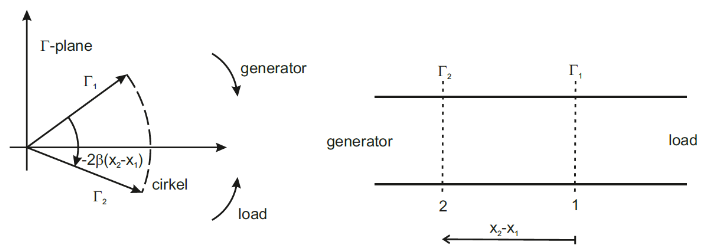
\includegraphics[width=0.8\linewidth]{../assets/chap03_prop2.png} %omg it contains the dutch 'cirkel' instead of 'circle', how did this book ever get published :|
					\caption{$\Gamma$ when moving on the transmission line}
					\label{fig:chap03_prop2}
				\end{figure}
				
			\subsubsection{Property 3}
				We normalize $Z_x$: $z_x = \frac{Z_x}{R_0}$. From here it follows that:
				\begin{equation}
					-\Gamma=\frac{y_x-1}{y_x+1}
				\end{equation}
				Here, $y_x = \frac{R_0}{Z_x} = \frac{Y_x}{G_0}$ is the normalized admittance. This means that we can find the admittance of a line easily on a smith chart by mirroring $\Gamma$ around the origin.
\end{document}
